Our proof approach closely follows classical proofs of the parametric BCLT, with
the key difference that we keep track of the data dependence in the residuals
(Chapter 10 of \citet{van:2000:asymptotic}, Theorem 1.4.2 of
\citet{ghosh:2003:bayesian}, and \citet{lehman:1983:pointestimation}). A
schematic of the proof setup is shown in \figref{proof_technique}, in which three
key regions, $R_1$, $R_2$ and $R_3$ are illustrated;
these regions are formally defined in \defref{region_division}
of \appref{bayes_clt_proof}.
As $N$ increases, we choose
the ball diameter $\delta$ small enough that three things happen:
%
\begin{itemize}[nosep]
\item $\likhat(\theta) \rightarrow \lik(\theta)$ uniformly within
$\thetaball{\delta}$ (primarily thanks to \assuref{bayes_clt}
\itemref{loglik_ulln});
\item $\likhat(\theta)$ remains strictly bounded away from $\likhat(\thetatrue)$ outside
$\thetaball{\delta}$ (primarily thanks to \assuref{bayes_clt} \itemref{strict_opt}); and
\item The posterior, which is proportional to $\exp(N \likhat(\theta))$, concentrates
in a region $R_1$ that shrinks at a rate slightly slower than $1/\sqrt{N}$.
\end{itemize}

\begin{figure}[h!]
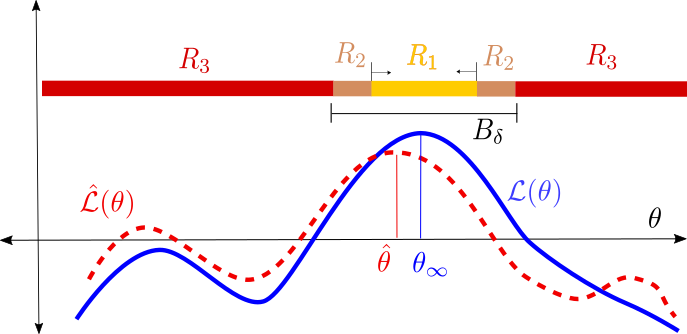
\includegraphics[width=\textwidth]{static_figures/BCLT_illustration.png}
\caption{Visual illustration of the proof technique.  As $N$ increases,
$\likhat(\theta) \rightarrow \lik(\theta)$
uniformly within $\thetaball{\delta}$, $\likhat(\theta)$ remains
bounded away from $\likhat(\thetatrue)$ outside of $\thetaball{\delta}$,
and the region $R_1$ that matters for the posterior shrinks at
a rate slightly slower than $1/\sqrt{N}$.}
\figlabel{proof_technique}
\end{figure}



Taking as given that the posterior concentrates in the shrinking region $R_1$,
we can fully characterize the posterior using Taylor series expansions within
the region $R_1$.  Our ability to form these Taylor series is guaranteed by the
differentiability conditions of \assuref{bayes_clt} \itemref{loglik_smooth} and
\defref{bclt_okay} \itemref{bclt_okay_as}.  Our ability to control the terms in
the Taylor series is guaranteed by uniform laws of large numbers (Chapter 19 of
\citet{van:2000:asymptotic}), which hold via \assuref{bayes_clt}
\itemref{loglik_ulln} and \defref{bclt_okay} \itemref{grad_op1}.

Finally, establishing that the posterior concentrates in $R_1$ requires separate
treatment of the region $R_2$, which is compact but adjacent to the region of
posterior concentration, and $R_3$, which encompasses the entire domain outside
of $\thetaball{\delta}$.  Thanks to uniform convergence within
$\thetaball{\delta}$, the region $R_2$ can be dealt with via Taylor expansions
and carefully choosing the shrinking rate of $R_1$.  However, the region $R_3$
requires a suite of additional assumptions to guarantee that the posterior does
not behave pathologically in the tails: namely, that $\likhat(\theta)$ remains
strictly bounded away from $\likhat(\thetatrue)$ (\assuref{bayes_clt}
\itemref{strict_opt}), that the prior is proper and bounded (\assuref{bayes_clt}
\itemref{prior_smooth,prior_proper}), and that average prior expectations of the
function of interest exist (\defref{bclt_okay} \itemref{prior_op1}).

We note that most of our assumptions about the prior (boundedness, propriety,
that certain prior expectations are bounded) serve only to establish that the
unbounded region $R_3$ does not contribute meaningfully to the posterior.
Inspection of the proof will reveal that weaker assumptions could also suffice,
at the cost of increased technical or notational complexity. For example, since
our analysis is asymptotic, one could assume only that the \emph{posterior}
satisfies \assuref{bayes_clt} \itemref{prior_smooth,prior_proper} and
\defref{bclt_okay} \itemref{prior_op1} with probability one after some finite
number of observations.  This posterior could then play the role of the prior in
the rest of the proof without modification.

In \appref{normal_example}, we verify our assumptions and prove the consistency
of the IJ covariance in the simple closed form example of inferring a univariate
normal mean with a misspecified variance.  This example, though simple, provides
intuition as well as a template for more complex settings.

